%!Tex Root = ../Main.tex
% ./Packete_und_Deklarationen.tex
\chapter{Ergebnisse und Ausblick}
\label{ch:ergebnisse_und_ausblick}

\section{Funktionsumfang}
\section{Qualitätssicherung}
% GCC + Execution entspricht einem einzigen großen Interpreter und beweist somit den linke Edge in 2.1
\label{sec:qualitätssicherung}
% RETI-Interpreter erwähnen
% TODO: zusammenfassendes Bild
\section{Kommentierter Kompiliervorgang}
\section{Erweiterungsideen}
Wenn eines Tages eine \colorbold{RETI-CPU} auf einem \colorbold{FPGA} implementiert werden sollte, sodass ein \colorbold{provisorisches Betriebssystem} darauf laufen könnte, dann wäre der nächste Schritt einen \colorbold{Self-Compiling Compiler} $C_{RETI\_PicoC}^{PicoC}$ (Defintion~\ref{def:self_compiling_compiler}) zu schreiben. Dadurch kann die \colorbold{Unabhängigkeit} von der Programmiersprache $L_Python$, in der der momentane Compiler $C_{PicoC}$ für $L_{PicoC}$ implementiert ist und die Unabhängigkeit von einer \colorbold{anderen Maschiene}, die bisher immer für das Cross-Compiling notwendig war erreicht werden.

\begin{Definition}{Self-compiling Compiler}{self_compiling_compiler}
  Compiler $C_w^w$, der in der Sprache $L_w$ \colorbold{geschrieben} ist, die er \colorbold{selbst} kompiliert. Also ein Compiler, der sich \colorbold{selbst} kompilieren kann.
\end{Definition}

Will man nun für eine Maschiene $M_{RETI}$, auf der bisher keine anderen Programmiersprachen mittels \colorbold{Bootstrapping} (Definition~\ref{def:bootstrapping}) zum laufen gebracht wurden, den gerade beschriebenen \colorbold{Self-compiling Compiler} $C_{RETI\_PicoC}^{PicoC}$ implementieren und hat bereits den gesamtem \colorbold{Self-compiling Compiler} $C_{RETI\_PicoC}^{PicoC}$ in der Sprache  $L_{PicoC}$ geschrieben, so stösst man auf ein Problem, dass auf das \colorbold{Henne-Ei-Problem}\footnote{Beschreibt die Situation, wenn ein System sich selbst als \colorbold{Abhängigkeit} hat, damit es überhaupt einen \colorbold{Anfang} für dieses System geben kann. Dafür steht das Problem mit der \colorbold{Henne} und dem \colorbold{Ei} sinnbildlich, da hier die Frage ist, wie das ganze seinen Anfang genommen hat, da beides \colorbold{zirkular} voneinander abhängt.} reduziert werden kann. Man bräuchte, um den \colorbold{Self-compiling Compiler} $C_{RETI\_PicoC}^{PicoC}$ auf der \colorbold{Maschiene} $M_{RETI}$ zu kompilieren bereits einen kompilierten \colorbold{Self-compiling Compiler} $C_{RETI\_PicoC}^{PicoC}$, der mit der Maschienensprache $B_{RETI}$ läuft. Es liegt eine \colorbold{zirkulare Abhängigkeit} vor, die man nur auflösen kann, indem eine \colorbold{externe Entität} zur Hilfe nimmt.

Da man den gesamten \colorbold{Self-compiling Compiler} $C_{RETI\_PicoC}^{PicoC}$ nicht selbst komplett in der Maschienensprache $B_{RETI}$ schreiben will, wäre eine Möglichkeit, dass man den \colorbold{Cross-Compiler} $C_{PicoC}^{Python}$, den man bereits in der Programmiersprache $L_{Python}$ implementiert hat, der in diesem Fall einen \colorbold{Bootstrapping Compiler} (Definition~\ref{def:bootstrap_compiler}) darstellt, auf einer anderen Maschiene $M_{other}$ dafür nutzt, damit dieser den \colorbold{Self-compiling Compiler} $C_{RETI\_PicoC}^{PicoC}$ für die Maschiene $M_{RETI}$ kompiliert bzw. \colorbold{bootstraped} und man den kompilierten \colorbold{RETI-Maschiendencode} dann einfach von der Maschiene $M_{other}$ auf die Maschiene $M_{RETI}$ kopiert.\footnote{Im Fall, dass auf der Maschiene $M_{RETI}$ die Programmiersprache $L_{Python}$ bereits mittels \colorbold{Bootstrapping} zum Laufen gebracht wurde, könnte der \colorbold{Self-compiling Compiler} $C_{RETI\_PicoC}^{PicoC}$ auch mithife des \colorbold{Cross-Compilers} $C_{PicoC}^{Python}$ als \colorbold{externe Entität} und der Programmiersprache $L_{Python}$ auf der Maschiene $M_{RETI}$ selbst kompiliert werden.}

\begin{figure}[H]
  \centering
  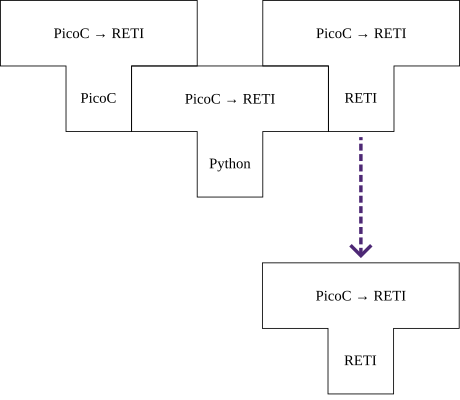
\includegraphics[width=0.5\linewidth]{./figures/cross_compiling.png}
  \caption{Cross-Compiler als Bootstrap Compiler}
\end{figure}

\begin{Special_Paragraph}
  Einen ersten \colorbold{minimalen Compiler} $C_{2\_w\_min}$ für eine Maschiene $M_2$ und Wunschsprache $L_w$ kann man entweder mittels eines \colorbold{externen} \colorbold{Bootstrap Compilers} $C_w^o$ kompilieren\footnote{In diesem Fall, dem \colorbold{Cross-Compiler} $C_{PicoC}^{Python}$.} oder man schreibt ihn direkt in der \colorbold{Maschienensprache} $B_2$ bzw. wenn ein \colorbold{Assembler} vorhanden ist, in der \colorbold{Assemblesprache} $A_2$.

  Die letzte Option wäre allerdings nur beim allerersten Compiler $C_{first}$ für eine allererste \colorbold{abstraktere Programmiersprache} $L_{first}$ mit Schleifen, Verzweigungen usw. notwendig gewesen. Ansonsten hätte man immer eine Kette, die beim allersten Compiler $C_{first}$ anfängt fortführen können, in der ein Compiler einen anderen Compiler kompiliert bzw. einen ersten minimalen Compiler kompiliert und dieser minimale Compiler dann eine umfangreichere Version von sich kompiliert usw.
\end{Special_Paragraph}

\begin{Definition}{Minimaler Compiler}{minimaler_compiler}
  Compiler $C_{w\_min}$, der nur die \colorbold{notwendigsten Funktionalitäten} einer Wunschsprache $L_w$, wie \colorbold{Schleifen},  \colorbold{Verzweigungen} kompiliert, die für die Implementierung eines \colorbold{Self-compiling Compilers} $C_{w}^{w}$ oder einer \colorbold{ersten Version} $C_{w_i}^{w_i}$ des Self-compiling Compilers $C_w^w$ wichtig sind.\footnote{Den \colorbold{PicoC-Compiler} könnte man auch als einen \colorbold{minimalen Compiler} ansehen.}
\end{Definition}

\begin{Definition}{Boostrap Compiler}{bootstrap_compiler}
  Compiler $C_w^o$, der es ermöglicht einen \colorbold{Self-compiling Compiler} $C_w^w$ zu \colorbold{boostrapen}, indem der Self-compiling Compiler $C_w^w$ mit dem \colorbold{Bootstrap Compiler} $C_w^o$ \colorbold{kompiliert} wird\footnote{Dabei kann es sich um einen \colorbold{lokal} auf der Maschiene selbst laufenden Compiler oder auch um einen \colorbold{Cross-Compiler} handeln.}. Der Bootstrapping Compiler stellt die  \colorbold{externe Entität} dar, die es ermöglicht die \colorbold{zirkulare Abhängikeit}, dass initial ein \colorbold{Self-compiling Compiler} $C_w^w$ bereits kompiliert vorliegen müsste, um sich selbst kompilieren zu können, zu brechen.
\end{Definition}

Aufbauend auf dem \colorbold{Self-compiling Compiler} $C_{RETI\_PicoC}^{PicoC}$, der einen \colorbold{minimalen Compiler} (Definition~\ref{def:minimaler_compiler}) für eine Teilmenge der \colorbold{Programmiersprache} C bzw. $L_C$ darstellt, könnte man auch noch weitere Teile der Programmiersprache $C$ bzw. $L_C$ für die Maschiene $M_{RETI}$ mittels \colorbold{Bootstrapping} implementieren.\footnote{Natürlich könnte man aber auch einfach den \colorbold{Cross-Compiler} $C_{PicoC}^{Python}$ um weitere Funktionalitäten von $L_C$ erweitern, hat dann aber weiterhin eine \colorbold{Abhängigkeit} von der Programmiersprache $L_{Python}$.}

Das bewerkstelligt man, indem man \colorbold{iterativ} auf der Zielmaschine $M_{RETI}$ selbst, aufbauend auf diesem \colorbold{minimalen Compiler} $C_{RETI\_PicoC}^{PicoC}$, wie in Subdefinition~\ref{def:bootstrapping}{.1} den minimalen Compiler schrittweise zu einem immer vollständigeren \colorbold{C-Compiler} $C_C$ weiterentwickelt.

\begin{Definition}{Bootstrapping}{bootstrapping}
  Wenn man einen \colorbold{Self-compiling Compiler} $C_{w}^{w}$ einer Wunschsprache $L_w$ auf einer \colorbold{Zielmaschine} $M$ zum laufen bringt\footnote{Z.B. mithilfe eines \colorbold{Bootstrap Compilers}.}\footnote{Der Begriff hat seinen Ursprung in der englischen \colorbold{Redewendung} \glqq pulling yourself up by your own bootstraps\grqq, was im deutschen ungefähr der aus den \colorbold{Lügengeschichten des Freiherrn von Münchhausen} bekannten Redewendung \glqq sich am eigenen Schopf aus dem Sumpf ziehen\grqq entspricht.}\footnote{Hat man einmal einen solchen \colorbold{Self-compiling Compiler} $C_{w}^{w}$ auf der Maschiene $M$ zum laufen gebracht, so kann man den Compiler auf der Maschiene $M$ weiterentwicklern, ohne von externen Entitäten, wie einer bestimmten Sprache $L_o$, in der der Compiler oder eine frühere Version des Compilers ursprünglich geschrieben war abhängig zu sein.}\footnote{Einen Compiler in der Sprache zu schreiben, die er selbst kompiliert und diesen Compiler dann sich selbst kompilieren zu lassen, kann eine gute \colorbold{Probe aufs Exempel} darstellen, dass der Compiler auch wirklich funktioniert.}. Dabei ist die Art von \colorbold{Bootstrapping} in \ref{def:bootstrapping}{.1} nochmal gesondert hervorzuheben:

  % https://tex.stackexchange.com/questions/7627/how-to-reference-paragraph
  \titleformat{\paragraph}[runin]{\normalfont\normalsize\bfseries}{}{0mm}{}[:]

  % https://tex.stackexchange.com/questions/7627/how-to-reference-paragraph
  \paragraph{\thetcbcounter{.1}}\label{par:bootstrapping}\hspace{-0.25cm}
  Wenn man die \colorbold{aktuelle Version} eines \colorbold{Self-compiling Compilers} $C_{w_i}^{w_i}$ der Wunschsprache $L_{w_i}$ mithilfe von \colorbold{früheren Versionen} seiner selbst kompiliert. Man schreibt also z.B. die aktuelle Version des Self-compiling Compilers in der Sprache $L_{w_{i-1}}$, welche von der früheren Version des Compilers, dem Self-compiling Compiler $C_{w_{i-1}}^{w_{i-1}}$ kompiliert wird und schafft es so \colorbold{iterativ} immer umfangreichere Compiler zu bauen.\footnote{Es ist hierbei theoretisch nicht notwendig den \colorbold{letzten} Self-compiling Compiler $C_{w_{i-1}}^{w_{i-1}}$ für das Kompilieren des \colorbold{neuen} Self-compiling Compilers $C_{w_i}^{w_i}$ zu verwenden, wenn z.B. der \colorbold{Self-compiling Compiler} $C_{w_{i-3}}^{w_{i-3}}$ auch bereits alle Funktionalitäten, die beim Schreiben des \colorbold{Self-compiling Compilers} $C_w^w$ verwendet werden kompilieren kann.}\footnote{Der Begriff ist sinnverwandt mit dem \colorbold{Booten} eines Computers, wo die wichtigste Software, der \colorbold{Kernel} zuerst in den Speicher geladen wird und darauf aufbauend von diesem dann das Betriebssysteme, welches bei Bedarf dann \colorbold{Systemsoftware}, Software, die das Ausführen von Anwendungssoftware ermöglicht oder unterstützt, wie z.B. Treiber. und \colorbold{Anwendungssoftware}, Software, deren Anwendung darin besteht, dass sie dem Benutzer unmittelbar eine Dienstleistung zur Verfügung stellt, lädt.}\footcite{earley_formalism_1970}
\end{Definition}

\begin{figure}[H]
  \centering
  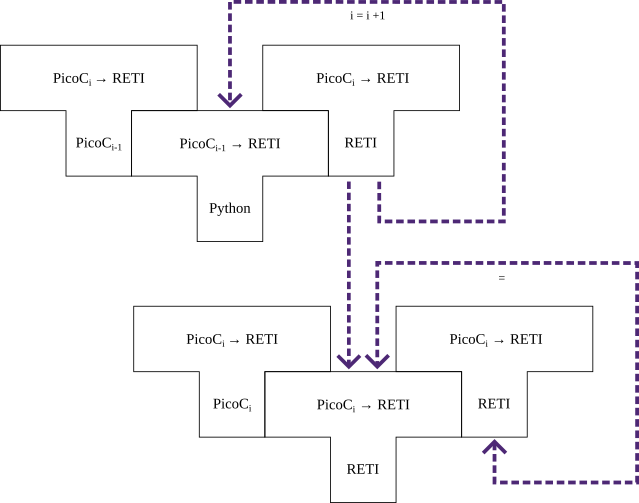
\includegraphics[width=0.66\linewidth]{./figures/bootstrapping.png}
  \caption{Iteratives Bootstrapping}
\end{figure}

\begin{Special_Paragraph}
  Auch wenn ein \colorbold{Self-compiling Compiler} $C_{w_i}^{w_i}$ in der Subdefinition~\ref{def:bootstrapping}{.1} selbst in einer früheren Version $L_{w_{i-1}}$ der Programmiersprache $L_{w_i}$ geschrieben wird, wird dieser nicht mit $C_{w_i}^{w_{i-1}}$ bezeichnet, sondern mit $C_{w_i}^{w_i}$, da es bei \colorbold{Self-compiling Compilern} darum geht, dass diese zwar in der Subdefinition~\ref{def:bootstrapping}{.1} eine frühere Version $C_{w_{i-1}}^{w_{i-1}}$ nutzen, um sich selbst kompilieren zu lassen, aber sie auch in der Lage sind sich selber zu kompilieren.
\end{Special_Paragraph}
